\chapter{Algorithmes quantiques}

\section{Algorithme de Deutsch-Jozsa}

Le problème de Deutsch-Jozsa s'intéresse à une fonction booléenne qui est soit équilibrée (ayant autant d'entrées à 1 qu'a 0), soit constante (toutes les entrées à 1, ou toutes les entrées à 0).

\begin{pb}[Deutsch-Jozsa]
Etant donnée une fonction $f$ booléenne qui est soit équilibrée, soit constante.
Le problème de Deutsch-Jozsa est de déterminer si $f$ est constante ou
équilibrée.  
\end{pb}

Dans le cas classique, il faut effectuer au pire $2^{n-1}+1$
évaluations pour déterminer si $f$ est constante ou équilibrée. Tout
d'abord, dès que deux évaluations sont différentes, $f$ est
nécessairement équilibrée. De plus, si après avoir évalué $2^{n-1}$
entrées et obtenu la même valeur, une évaluation supplémentaire nous
permet de connaitre dans quelle catégorie $f$ se trouve.

Dans le cas quantique, on peut résoudre ce problème en effectuant qu'une seule évaluation, parallèle, de $f$. Le schéma suivant illustre le fonctionnement de l'algorithme présente par Deutsch et Jozsa en 1992 \cite{Deutsch92}:

\begin{figure}[htbp]
    \centering
    \centerline{
        \Qcircuit @C=1em @R=.7em {
          & \lstick{\ket{0}^n} \barrier[-1.75em]{1} & \gate{H^{\otimes n}} \barrier[-1.5em]{1} & \multigate{1}{U_f} \barrier[-1.75em]{1} & \gate{H^{\otimes n}} \barrier[-1.5em]{1} & \meter \\
          & \lstick{\ket{1}} & \gate{H} & \ghost{U_f} & \qw & \\
          \hspace{3em} \ket{u_{0}} & \hspace{9em} \ket{u_{1}} &  \hspace{10em} \ket{u_{2}} & \hspace{10em} \ket{u_{3}}
        }
    }
    \caption{Schéma de l'algorithme}
    \label{fig:univerise}
\end{figure}

Les détails algébriques de l'algorithme sont disponibles en annexes.
\medbreak
On dispose au départ un (n+1)-qubit, c'est à dire (n+1) qubits associés, les n premiers mis à 0 et le dernier mis à 1. Cet état d'entrée $\ket{u_0}$ est construit préalablement, puis est donné en entrée à des portes de Hadamard. Pour rappel, cette porte permet de faire passer un qubit d'un état pur ($\ket{0}$ ou $\ket{1}$) à un état équilibré. 

Au sortir de cette porte, on obtient l'état $\ket{u_1}$, qui si mesuré va nous donner avec autant de probabilité un des états purs. On le passe donc à la "boite" $U_f$. On appelle ce bloc \textbf{oracle}, qui implémente la fonction $f$ qu'on souhaite évaluer pour $n$ qubits (on ne détaille pas ici la façon d'implémenter $f$). L'entrée étant un (n+1)-qubit équilibré, l'oracle va évaluer en simultané toutes les entrées, correspondant aux états purs superposés. C'est ici qu'on peut à nouveau montrer la force de l'informatique quantique: avec en entrée un état superposé, un bloc fonctionnel va faire évoluer le système en effectuant le calcul pour tout les états purs superposés composant l'entrée.

On obtient $\ket{u_2}$, qui contient la solution de notre problème. Néanmoins, si on essaye ici de mesurer le système, on ne va pas obtenir directement une réponse "oui" ou "non" à notre problème: le système est encore dans un état superposé, et la réponse est codée dans les modules associés aux états purs superposés. Si on mesure $\ket{u_2}$, on obtiendra aléatoirement un des état purs composant le système.

Pour résoudre ce problème, on applique à nouveau une porte de Hadamard pour obtenir un $\ket{u_3}$. On l'a dit précédement, quand appliqué à un état pur, la porte de Hadamard permet de créer un état équilibré. En revanche, quand comme ici on l'applique à un état déjà superposé, on peut obtenir directement un état qui va nous donner à coup sûr une réponse binaire. Ici, quand on va mesurer $\ket{u_3}$, on va soit mesurer un mot binaire de $n$ bits valant 0, et dans ce cas la fonction est constante. Si on obtient n'importe quelle autre solution, alors la fonction est équilibrée. A nouveau, les détails algébriques de cet algorithme sont disponibles en annexes.

\medbreak

Cet algorithme permet principalement de prouver la supériorité de l'informatique quantique sur ce type de problèmes: on arrive effectivement à atteindre des performances qui sont inatteignables avec des ordinateurs classiques. Plusieurs autres algorithmes ont été créés en se basant sur celui-là, en modifiant le problème et la fonction évaluée, mais en gardant l'algorithme. On peut notamment citer l'algorithme de Bernstein-Vazirani \cite{Bernstein97} qui permet de résoudre un problème d'arithmétique modulaire.

\section{Algorithme de Grover}

On s'intéresse maintenant à un problème classique d'informatique: la recherche dans des listes. En informatique classique, on connait un certain nombre d'algorithmes pour effectuer des recherches dans des listes, qu'elles soient triées ou non triées.

\begin{pb}[Grover]
Soit une liste non triée à $N$ entrées. Le problème de Grover est de rechercher une entrée spécifique dans cette liste de façon efficace.
\end{pb}

Classiquement, l'algorithme le plus efficace devra effectuer au pire $N$ itérations sur la liste pour trouver l'élément voulu. La liste étant non triée, on ne peut pas utiliser des algorithmes qui divisent la liste, qui permettent d'obtenir des performances en $\mathcal{O}(\log N)$.

En utilisant les principes de l'informatique quantique, Lou Grover a proposé en 1992 \cite{Grover96} un algorithme permettant de trouver la solution avec une forte probabilité, en juste $\mathcal{O}(\sqrt N)$

\begin{figure}[htbp]
  \centering
  \centerline{
      \Qcircuit @C=1em @R=.7em {
        & & & & & \mbox{Grover operator: Repeat $\mathcal{O}(\sqrt N)$ times} \\
        & \lstick{\ket{0}^n} \barrier[-1.75em]{1}  & \gate{H^{\otimes n}} \barrier[-1.75em]{1} & \multigate{1}{U_w} \barrier[-1.5em]{1} & \multigate{1}{U_s} \barrier[-1.25em]{1} & \meter \\
        & \lstick{\ket{1}} & \gate{H} & \ghost{U_w} &  \ghost{U_s} & \qw & \\
        \hspace{3em} \ket{u_{0}} & \hspace{8em} \ket{u_{1}} &  \hspace{10em} \ket{u_{2}} & \hspace{10em} \ket{u_{3}} \gategroup{2}{4}{3}{5}{.7em}{^\}}
      }
    }
  \caption{Schéma de l'algorithme}
  \label{fig:univerise}
\end{figure}

De même que pour Deutsch-Jozsa, les détails algébriques de cet algorithme sont disponibles en annexes.

On commence donc de la même manière avec n qubits initialisés à $\ket{0}$ et 1 à $\ket{1}$, et on les passe tous dans une porte de Hadamard pour avoir des qubits équilibrés, afin de faire un traitement parallèle.

La deuxième étape consiste à appliquer l'opérateur de Grover à l'état superposé $\ket{u1}$. On vient effectuer deux opérations successives ici.

\begin{enumerate}
  \item Une opération d'inversion d'amplitude avec l'opérateur $U_w$. On a au départ les $n$ états purs superposés de façon équilibrés, ils ont donc tous la même amplitude (le module devant l'état pur). Cet opérateur vient inverser l'amplitude de l'état pur qu'on cible. On se retrouve après dans un état équilibré, puisque les probabilités sont les amplitudes mises au carrés. On a donc la réponse dans l'état quantique, mais elle est inaccessible à la mesure.
  \item Une opération de miroir à la moyenne avec l'opérateur $U_s$. Cet opérateur vient calculer la moyenne des amplitudes, puis enlever aux amplitudes leur différence à la moyenne. Dans le cas des amplitudes qui n'ont pas bougé avec $U_w$, on se retrouve légèrement en dessous de la moyenne, et dans le cas de l'état ciblé, on se retrouve bien au dessus de la moyenne.
\end{enumerate}

\pgfplotstableread[row sep=\\,col sep=&]{
    state & amplitude \\
    $\ket{000}$ & 0.35355  \\
    $\ket{001}$ & 0.35355  \\
    $\ket{010}$ & 0.35355  \\
    $\ket{011}$ & 0.35355  \\
    $\ket{100}$ & 0.35355  \\
    $\ket{101}$ & 0.35355  \\
    $\ket{110}$ & 0.35355  \\
    $\ket{111}$ & 0.35355  \\
}\afterHadamard
\pgfplotstableread[row sep=\\,col sep=&]{
    state & amplitude \\
    $\ket{000}$ & 0.35355  \\
    $\ket{001}$ & 0.35355  \\
    $\ket{010}$ & -0.35355  \\
    $\ket{011}$ & 0.35355  \\
    $\ket{100}$ & 0.35355  \\
    $\ket{101}$ & 0.35355  \\
    $\ket{110}$ & 0.35355  \\
    $\ket{111}$ & 0.35355  \\
}\afterUw
\pgfplotstableread[row sep=\\,col sep=&]{
    state & amplitude \\
    $\ket{000}$ & 0.176  \\
    $\ket{001}$ & 0.176  \\
    $\ket{010}$ & 0.884  \\
    $\ket{011}$ & 0.176  \\
    $\ket{100}$ & 0.176  \\
    $\ket{101}$ & 0.176  \\
    $\ket{110}$ & 0.176  \\
    $\ket{111}$ & 0.176  \\
}\afterUs

\begin{figure*}[t!]
  \centering
  \begin{subfigure}[t]{0.33\textwidth}
      \centering
      \begin{tikzpicture}[scale=0.55]
        \begin{axis}[
                ybar,
                symbolic x coords={$\ket{000}$, $\ket{001}$, $\ket{010}$, $\ket{011}$, $\ket{100}$, $\ket{101}$, $\ket{110}$, $\ket{111}$},
                xtick=data,
            ]
            \addplot table[x=state,y=amplitude]{\afterHadamard};
        \end{axis}
      \end{tikzpicture}
      \caption{$\ket{u_1}$}
  \end{subfigure}%
  \begin{subfigure}[t]{0.33\textwidth}
      \centering
      \begin{tikzpicture}[scale=0.55]
        \begin{axis}[
                ybar,
                symbolic x coords={$\ket{000}$, $\ket{001}$, $\ket{010}$, $\ket{011}$, $\ket{100}$, $\ket{101}$, $\ket{110}$, $\ket{111}$},
                xtick=data,
            ]
            \addplot table[x=state,y=amplitude]{\afterUw};
        \end{axis}
      \end{tikzpicture}
      \caption{$\ket{u_2}$}
  \end{subfigure}
  \begin{subfigure}[t]{0.33\textwidth}
    \centering
    \begin{tikzpicture}[scale=0.55]
      \begin{axis}[
              ybar,
              symbolic x coords={$\ket{000}$, $\ket{001}$, $\ket{010}$, $\ket{011}$, $\ket{100}$, $\ket{101}$, $\ket{110}$, $\ket{111}$},
              xtick=data,
          ]
          \addplot table[x=state,y=amplitude]{\afterUs};
      \end{axis}
    \end{tikzpicture}
    \caption{$\ket{u_3}$}
  \end{subfigure}
  \caption{Evolution des amplitudes pour $n=3$ qubits}
\end{figure*}

Cette figure illustre cette évolution pour 3 qubits. On voit qu'a la fin de $U_s$, on obtient un état quantique qui a une forte probabilité de tomber sur l'état voulu (ici, $\ket{010}$), les amplitudes de ceux qu'on ne veut pas ayant été fortement réduites. Néanmoins, on est toujours pas sûr de tomber sur le bon résultat: dans ce cas précis, la probabilité de tomber sur $\ket{010}$ est d'environ 78\%, on a quand même quasiment 20\% de chances de mesurer un autre état. Ce n'est pas satisfaisant.

La solution est de réappliquer les portes $U_w$ et $U_s$. Ceci va encore plus diminuer les probabilités des états non voulus et augmenter la probabilité de l'état voulu.
On peut prouver, notamment géométriquement, que le nombre d'optimal d'itérations est $\frac{\pi}{4}\sqrt{N}$. En fait, il se passe autre chose: si on dépasse ce nombre optimal d'itération, on va diminuer l'amplitude de l'état voulu et augmenter les probabilités des autres états: c'est cyclique. La figure suivante illustre une simulation sur plus d'itérations que ce qui est necessaire:

\begin{figure}[htbp]
  \centering
  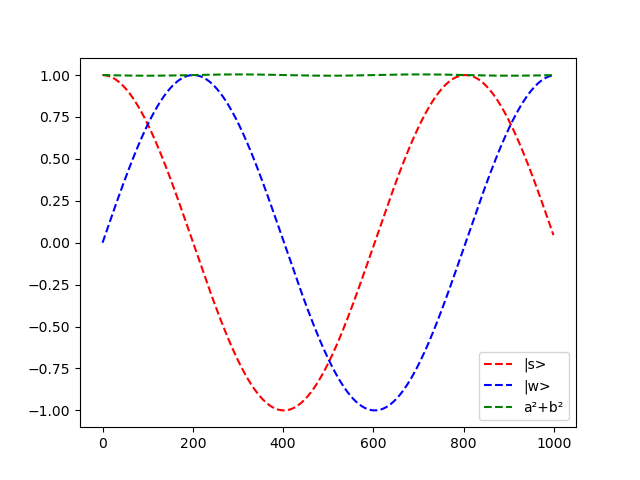
\includegraphics[scale=0.3]{Grover/grover_n16_1000.png}
  \caption{Evolution des amplitudes pour n=16, sur 1000 itérations}
\end{figure}

En bleu, on représente la probabilité de tomber sur l'état cible, en rouge la probabilité de tomber sur un autre état (en vert, pour indication, la somme des probabilités pour vérifier que la somme vaut bien 1). On voit bien ici le rebouclement après $\frac{\pi}{4}\sqrt{N}$ itérations.

\section{Algorithme de Shor}

On peut enfin étudier l'algorithme de Shor, proposé par Peter Shor en 1997 \cite{Shor97}.

\begin{pb}
  On s'intéresse au problème de la factorisation d'un nombre $N=q \times q$ avec $p$ et $q$ nombres entiers très grands.
\end{pb}

Classiquement, ce problème est résolvable en $\mathcal{O}(\exp{[c . n^{\frac{1}{3}} (\log n)^{\frac{2}{3}} ]})$ avec l'algorithme du crible du corps algébrique. Cet algorithme est certes efficace pour des nombres supérieurs à $10^{100}$, mais ne permet pas de factoriser pour des nombres de $2048$ ou $4096$ bits. Ce domaine de recherche avance rapidement, et de nouveaux algorithmes sont trouvés permettant d'améliorer les performances. On ne trouve en revanche toujours pas d'algorithmes permettant de résoudre ce problème en un temps polynomial.

En utilisant l'informatique, Shor a démontré que ce problème était résolvable bien plus rapidement avec un processeur quantique, en un peu plus rapidement que $\mathcal{O}(n^3)$. En fait, Shor résout avec son algorithme une sous-partie d'un algorithme:

\begin{algorithm}[H]
  \SetAlgoLined
  \KwData{N}
  \Repeat{}{
    choose a coprime with N;

    find smallest r such that $a^r \equiv 1 (mod N)$;

    \eIf{r is even}
    {
      $x \equiv a^{\frac{r}{2}} (mod N) $;

      \eIf{$x + 1 \not \equiv 0 (mod N)$}
      {
        at least one of $\{p, q\} \in \{gcd(x+1, N), gcd(x-1, N)\}$;

        break;
      }
      {
        continue;
      }
    }
    {
      continue;
    }
  }
\end{algorithm}

Cet algorithme permet de trouver les facteurs premiers $p$ et $q$. On peut prouver que la deuxième instruction revient à chercher la période de la fonction $a^r \Mod{N}$. C'est cette instruction spécifique qui est compliquée à résoudre classiquement, mais que Shor à réussi à résoudre en quantique.

Cet algorithme se passe en 3 étapes. Les deux premières sont similaires aux deux algorithmes précédents: on fait passer un n-qubit de l'état $\ket{0}^{\otimes n}$ à l'état équilibré; puis on évalue la fonction $a^r \Mod{N}$ pour l'état équilibré. La troisième étape fait intervenir une nouvelle notion: la transformée de Fourier quantique. C'est une généralisation de la porte de Hadamard, qui fait passer les qubits de la base $\{\ket{0}, \ket{1}\}$ à la base $\{\ket{+}, \ket{-}\}$ (pour rappel, on a $\ket{+} = \frac{1}{\sqrt{2}}(\ket{0} + \ket{1})$, et $\ket{-} = \frac{1}{\sqrt{2}}(\ket{0} - \ket{1})$).

La transformée de Fourier quantique peut être comprise ici en faisant l'analogie à la version classique. Dans un cas classique, quand on a une fonction périodique, l'application de la transformée de Fourier permet de passer de la représentation temporelle à la représentation fréquentielle. Sur cette représentation, on obtient des raies de Dirac aux fréquences correspondant aux périodes de la fonction. Il suffit alors de lire les valeurs pour obtenir les périodes. Il s'agit du même principe en quantique: la transformée de Fourier quantique nous permet d'obtenir directement la valeur de la période, avec l'avantage de faire le calcul parallélisé.

\medbreak

Cet algorithme a déjà été implémenté sur de réels processeurs quantique, permettant de factoriser 15 en 5 et 3 en 2001 \cite{Vandersypen01}, puis de factoriser 21 en 3 et 7 en 2011 \cite{Martin11}. Aucun travail expérimental n'a réussi à ce jour à factoriser des nombres plus grands que ça, limitant les risques potentiels à la cybersécurité engendrés par cet algorithme. La structure de la solution de Shor necessite en effet beaucoup de corrections d'erreur sur les mises en oeuvres pratiques dûes au bruits sur les grand nombres de portes utilisées, ce qui complexifie et ralentis les implémentations.

En revanche, ce problème de factorisation n'a pas pour seule solution celle proposée par Shor, et notamment une implémentations théorique de 2018 montre une factorisation d'entiers de 2048 bits en 8 heures, en utilisant 20 million de qubits \cite{gidney2019factor}. D'autres algorithmes sont présentés depuis 2010 notamment, présentant d'autres alternatives à Shor \cite{anschuetz2018variational}.